\documentclass[10pt]{beamer}
\usetheme[] {Feather}
  
%-------------------------------------------------------
% PACKAGES
%-------------------------------------------------------

\usepackage[utf8]{inputenc}
\usepackage[english]{babel}
\usepackage[T1]{fontenc}
\usepackage{helvet}
\usepackage{amsmath}
\usepackage{amssymb}
\usepackage{mathrsfs}
\usepackage{graphicx}
\usepackage{pdfpages}
\usepackage{tikz}
\usepackage{physics}
\usepackage{realboxes}
\usepackage{siunitx}
\usepackage{pifont}
\usepackage{tikz}

\definecolor{cec1d24}{RGB}{236,29,36}
\definecolor{cffffff}{RGB}{255,255,255}
\def\Put(#1,#2)#3{\leavevmode\makebox(0,0){\put(#1,#2){#3}}}


%-------------------------------------------------------
% DEFFINING AND REDEFINING COMMANDS
%-------------------------------------------------------

% colored hyperlinks
\newcommand{\chref}[2]{
  \href{#1}{{\usebeamercolor[bg]{Feather}#2}}
}
\newcommand\blfootnote[1]{%
  \begingroup
  \renewcommand\thefootnote{}\footnote{#1}%
  \addtocounter{footnote}{-1}%
  \endgroup
}
%-------------------------------------------------------
% INFORMATIONS SUR LA PAGE DE TITRE
%-------------------------------------------------------


\title[ Preparing the charge readout plane of the $6 \times 6 \times \SI{6}{\meter\cubed}$  and analyzing the performances of the $3 \times 1 \times \SI{1}{\meter\cubed}$ of DLArTPC detector of WA105]{
\vspace{3cm}
      \textbf{ Preparing and testing the charge readout plane of the  \texorpdfstring{$6 \times 6 \times \SI{6}{\meter\cubed}$}{666} demonstrator and analyzing the performances of the  \texorpdfstring{$3 \times 1 \times \SI{1}{\meter\cubed}$}{311} prototype of double phase liquid argon TPC detector of WA105} \\
}
\author[Philippe COTTE]
{
    Philippe COTTE
}
\date{April 5th 2019}

%-------------------------------------------------------
% CORPS DE LA PRESENTATION
%-------------------------------------------------------

\begin{document}

%-------------------------------------------------------
% PAGE DE TITRE
%-------------------------------------------------------

{\1% % this is the name of the PDF file for the background
    \begin{frame}[plain,noframenumbering] % the plain option removes the header from the title page, noframenumbering removes the numbering of this frame only
        \titlepage % call the title page information from above
    \end{frame}}
    
    \begin{frame}{Context}{Neutrino oscillations : main questions}
    	\begin{scriptsize}
    	\begin{minipage}{0.48\textwidth}
    			Neutrinos can change flavor through PMNS matrix $\Rightarrow$ they have mass\\
    			
	    		 $
		    		 \left(\begin{matrix}
		    		 \nu_e \\ \nu_{\mu} \\ \nu_{\tau}
		    		 \end{matrix}\right) =
		    		 \left(\begin{matrix}
		    		 U_{e1} & U_{e2} & \textcolor{red}{U_{e3}} \\
		    		 \textcolor{red}{U_{\mu 1}} & \textcolor{red}{U_{\mu 2}} & U_{\mu 3}  \\
		    		 \textcolor{red}{U_{\tau 1}} & \textcolor{red}{U_{\tau 2}} & U_{\tau 3} 
		    		 \end{matrix}\right)
		    		 \left(\begin{matrix}
		    		 \nu_1 \\ \nu_2 \\ \nu_3
		    		 \end{matrix}\right)
	    		$\\
	    		
	    		Probability to change flavor : \\
	    		$
		    		P(\nu_{\mu}\to\nu_e) = $ \\ 
	    		$
		    		- 4\sum_{i>j}\Re(U_{\mu i}U_{e i}^*U_{\mu j}^*U_{e j})\sin^2\left(\textcolor{blue}{\Delta m_{ij}^2}\frac{L}{4E}\right) $\\
	    		$
		    		 +2\sum_{i>j}\Im(U_{\mu i}U_{e i}^*U_{\mu j}^*U_{e j})\sin\left(\textcolor{blue}{\Delta m_{ij}^2}\frac{L}{2E}\right)
    		   $ \\
    		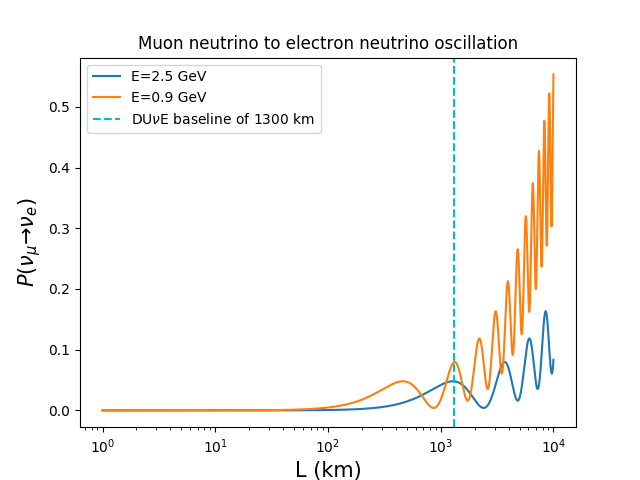
\includegraphics[width=\textwidth]{figures/contexte/numu-nue-vs-L-3flav.png}
    	\end{minipage}
    	\hfill
    	\begin{minipage}{0.48\textwidth}
    		\begin{itemize}
    			\item[$\bullet$] $\textcolor{red}{U_{\alpha i}}$ terms contain $e^{i\delta_{CP}}$
    			\item[$\bullet$] If $\delta_{CP} \ne 0$ and $\pi$: $P(\nu_{\mu}\to\nu_e) \ne P(\overline{\nu}_{\mu}\to\overline{\nu}_e)$
    		\end{itemize}
    		$\Rightarrow$ Possible \textcolor{red}{CP violation} in leptonic sector \\ 
    		$\Rightarrow$ could explain matter-antimatter asymmetry in the universe\\
	    	
	    	\begin{itemize}
	    		\item[$\bullet$]$\textcolor{blue}{\Delta m_{ij}^2} = m_i^2-m_j^2$
	    		\item[$\bullet$] $\Delta m_{21(sol)}^2\simeq \SI{e-5}{\electronvolt\squared}$
	    		\item[$\bullet$] $|\Delta m_{31(atm)}^2| \simeq |\Delta m_{32}^2| \simeq \SI{e-3}{\electronvolt\squared}$
	    	\end{itemize}
	    	$\Rightarrow$ Unknown \textcolor{blue}{mass hierarchy} : \\
	    	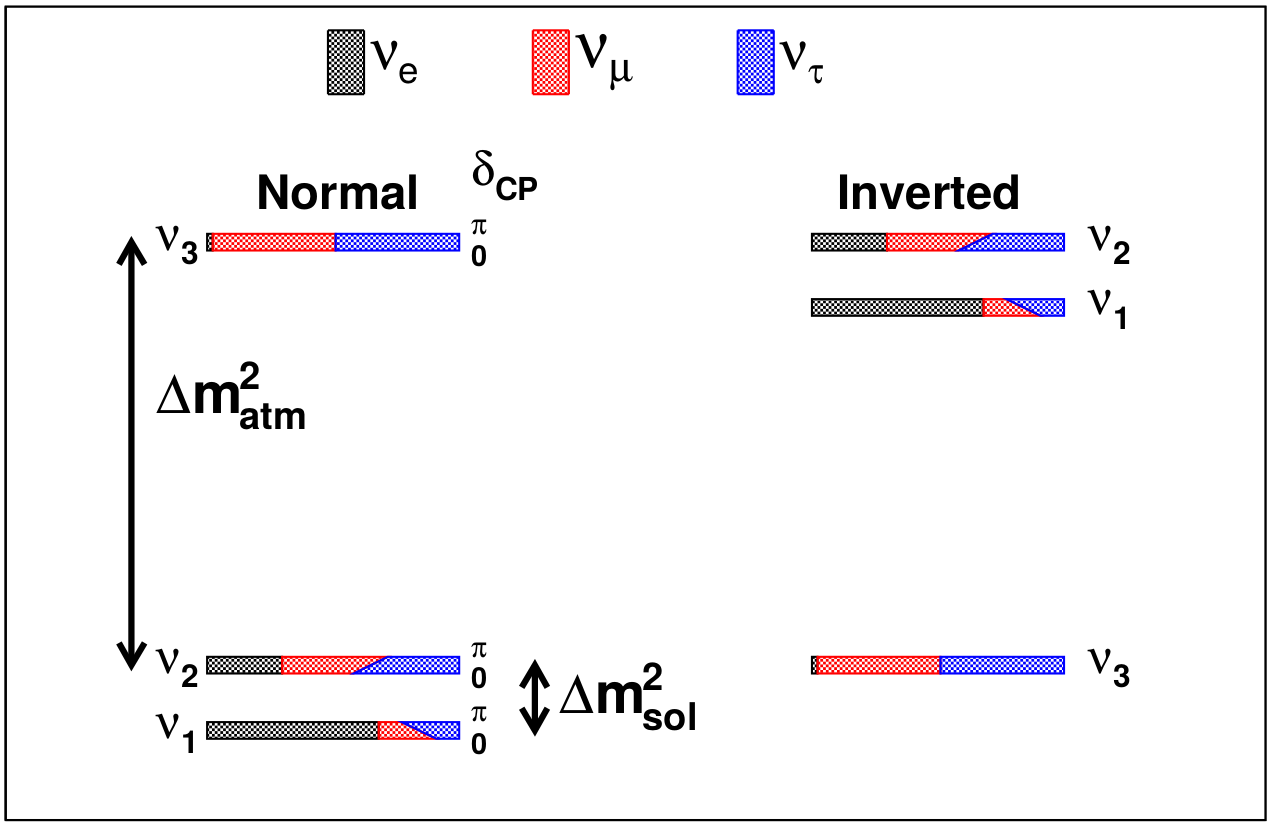
\includegraphics[width=0.8\textwidth]{figures/contexte/mass_hierarchy.png}\\
	    	Many BSM theories depend on  \textcolor{blue}{MH}
	    \end{minipage}
	\end{scriptsize}
	    
    \end{frame}
    
    \begin{frame}{Context}{DU$\nu$E : a longue baseline neutrino oscillation experiment}
    	\begin{scriptsize}
    	\begin{minipage}{0.58\textwidth}
    		The Deep Underground Neutrino Experiment:\\
    		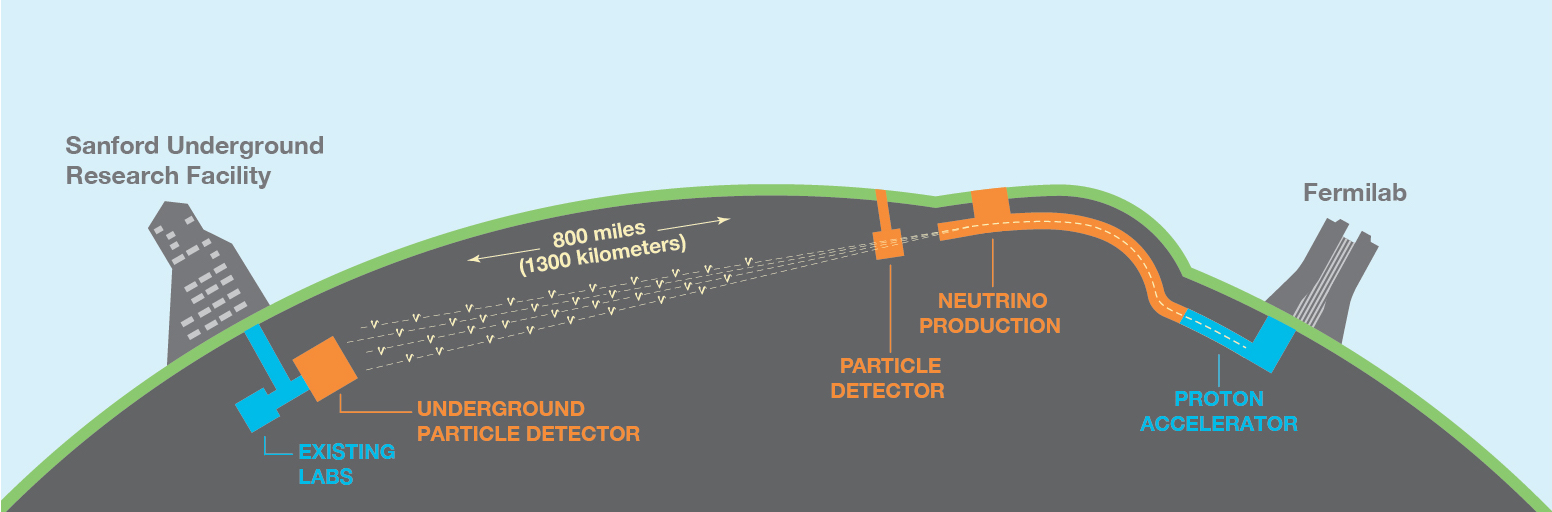
\includegraphics[width=\textwidth]{figures/contexte/dune.jpg}\\
    		
    		1 of the 4 far detector modules:\\
    		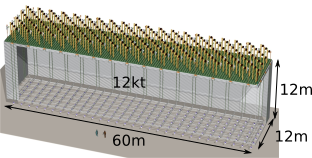
\includegraphics[width=\textwidth]{figures/contexte/dune_module.png}\\
    	\end{minipage}
    	\hfill
    	\begin{minipage}{0.38\textwidth}
    		\begin{itemize}
    			\item[$\bullet$]Baseline: \SI{1300}{\kilo\meter}
    			\item[$\bullet$]Beam energy: $0.5$--\SI{5}{\giga\electronvolt} $\Rightarrow$~Can cover 2 oscillation maxima
    			\item[$\bullet$]Can send $\nu_{\mu}$ or $\overline{\nu}_{\mu}$
    			\item[$\bullet$] Matter effects allow direct MH probing
    			\item[$\bullet$] $2^{nd}$ oscillation maximum less sensitive to matter effects $\Rightarrow$~More sensitive to $\delta_{CP}$
    		\end{itemize}
	    \end{minipage}
	\end{scriptsize}
    \end{frame}
    
    \begin{frame}{Context}{DU$\nu$E's detector technology}
    	\begin{scriptsize}
    		\begin{minipage}{0.48\textwidth}
    			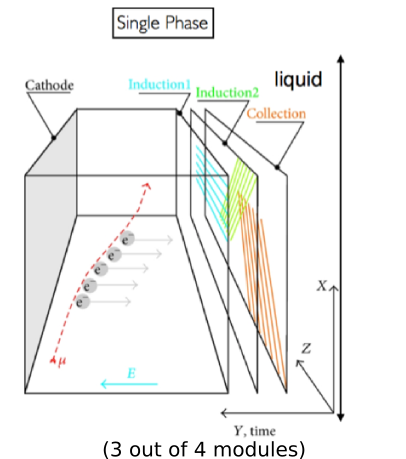
\includegraphics[width=\textwidth]{figures/contexte/lartpc.png}\\
    		\end{minipage}
    		\hfill
    		\begin{minipage}{0.48\textwidth}
    			Advantages of a Time Projection Chamber:    			
    			\begin{itemize}
    				\item[$\bullet$] 3D information at \si{\milli\meter} precision
    				\item[$\bullet$] Big volumes
    				\item[$\bullet$] Calorimetry
    				\item[$\bullet$] Particle Identification
    			\end{itemize}    			
    			Largest LArTPC that detected neutrinos: ICARUS (\SI{600}{\tonne})\\
    			
    			Why Liquid argon?
    			\begin{itemize}
    				\item[$\bullet$] Cheap and abundant
    				\item[$\bullet$] Scintillate at ionization (used for trigger)
    				\item[$\bullet$] Is inert: does not absorb electrons
    				\item[$\bullet$] Is dense: ideal for neutrino physics
    				\item[$\bullet$] Lots of electrons created at ionization
    			\end{itemize}
    		\end{minipage}
    	\end{scriptsize}
    	
    \end{frame}
    
    \begin{frame}{Context}{DU$\nu$E's detector technology}
    	\begin{scriptsize}
    		\begin{minipage}{0.48\textwidth}
    			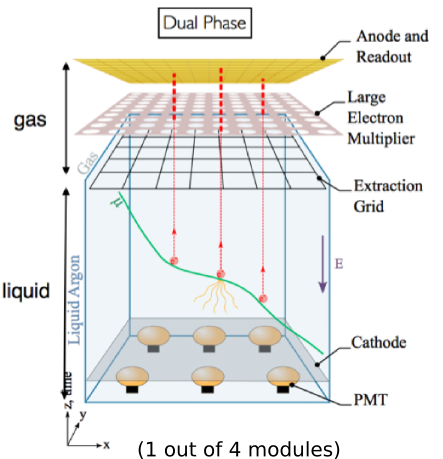
\includegraphics[width=\textwidth]{figures/contexte/dlartpc.png}\\
    		\end{minipage}
    		\hfill
    		\begin{minipage}{0.48\textwidth}
    			Double phase version: Amplification of the signal in gas
    			\begin{itemize}
    				\item[$\bullet$] Allows lower energy threshold
    				\item[$\bullet$] Allows smaller readout pitch: better 2D resolution
    				\item[$\bullet$] Allows bigger drift lengths: less dead volumes
    				\item[$\bullet$] High signal/noise ratio
    			\end{itemize}    			
    			DLArTPC are young: biggest one is \SI{250}{\liter}\\
    		\end{minipage}
    	\end{scriptsize}
    	$\Rightarrow$ need an extra step of R\&D to reach DU$\nu$E's scale
    \end{frame}
    
    \begin{frame}{The \texorpdfstring{$6 \times 6 \times \SI{6}{\meter\cubed}$}{666}
    		\begin{scriptsize}
    		\end{scriptsize} demonstrator}{Tonne-scale and \si{\meter\squared} readout planes chalenges}
	    Photo of 666 with CRP, LEM and anode, objectives, Irfu missions
    \end{frame}
    
    \begin{frame}{The \texorpdfstring{$6 \times 6 \times \SI{6}{\meter\cubed}$}{666}
    		\begin{scriptsize}
    		\end{scriptsize} demonstrator}{Gain in LEM-Anode sandwich}
    	Formula, 3L plot, photos and schematics, design from 3L measurements
    \end{frame}
    
    \begin{frame}{The \texorpdfstring{$6 \times 6 \times \SI{6}{\meter\cubed}$}{666}
    		\begin{scriptsize}
    		\end{scriptsize} demonstrator}{Study of LEM's dead zones}
    	Motivation, geom, plot (border only, easier to understand)
    \end{frame}
    
    \begin{frame}{The \texorpdfstring{$6 \times 6 \times \SI{6}{\meter\cubed}$}{666}
    		\begin{scriptsize}
    		\end{scriptsize} demonstrator}{Study of extraction and induction fields effect on collected charge}
    	Motivation, method, ansys plot
    \end{frame}
    
    \begin{frame}{The \texorpdfstring{$6 \times 6 \times \SI{6}{\meter\cubed}$}{666}
    		\begin{scriptsize}
    		\end{scriptsize} demonstrator}{Study of extraction and induction fields effect on collected charge}
    	drift plot, drift histogram, coll proba maps
    \end{frame}
    
    \begin{frame}{The \texorpdfstring{$6 \times 6 \times \SI{6}{\meter\cubed}$}{666}
    		\begin{scriptsize}
    		\end{scriptsize} demonstrator}{LEM tests in high pressure chamber at Saclay : High voltage}
    	photos, say that we showed that original design could ot reach high voltages so made a new one
    \end{frame}
    
    \begin{frame}{The \texorpdfstring{$6 \times 6 \times \SI{6}{\meter\cubed}$}{666}
    		\begin{scriptsize}
    		\end{scriptsize} demonstrator}{LEM tests in high pressure chamber at Saclay : gain measurements}
    	Photo and plots
    \end{frame}
    
    \begin{frame}{The \texorpdfstring{$6 \times 6 \times \SI{6}{\meter\cubed}$}{666}
    		\begin{scriptsize}
    		\end{scriptsize} demonstrator}{LEM thickness measurements}
    	Motivations and procedure
    \end{frame}
    
    \begin{frame}{The \texorpdfstring{$6 \times 6 \times \SI{6}{\meter\cubed}$}{666}
    		\begin{scriptsize}
    		\end{scriptsize} demonstrator}{LEM thickness measurements}
    	Results and predicted impact on gain
    \end{frame}
    
    \begin{frame}{The \texorpdfstring{$6 \times 6 \times \SI{6}{\meter\cubed}$}{666}
    		\begin{scriptsize}
    		\end{scriptsize} demonstrator}{Full CRP high tests in cold box}
    	Photos and results table. Carbonization : developing a different etching technique in Rui DeOlivera's lab at CERN
    \end{frame}
    
    \begin{frame}{The \texorpdfstring{$3 \times 1 \times \SI{1}{\meter\cubed}$}{311}
    		\begin{scriptsize}
    		\end{scriptsize} prototype}{Goals}
    	Photos, goals, difficulties, event display
    \end{frame}
    
    \begin{frame}{The \texorpdfstring{$3 \times 1 \times \SI{1}{\meter\cubed}$}{311}
    		\begin{scriptsize}
    		\end{scriptsize} prototype}{Purity and electron lifetime}
    	Plots and fit
    \end{frame}
    
    \begin{frame}{The \texorpdfstring{$3 \times 1 \times \SI{1}{\meter\cubed}$}{311}
    		\begin{scriptsize}
    		\end{scriptsize} prototype}{Charging up}
    	plots and comments
    \end{frame}
    
    \begin{frame}{The \texorpdfstring{$3 \times 1 \times \SI{1}{\meter\cubed}$}{311}
    		\begin{scriptsize}
    		\end{scriptsize} prototype}{Gain}
    	Current plots, say missing points have high noise because low extraction field, dvping a new soft to analyze them
    \end{frame}
    
\end{document}

